\documentclass[a4paper,12pt,titlepage]{article} % [papersize,fontsize,add title page]{document type}

% This LaTeX file can be turned straight into a pdf by "PDFTeXify" in WinEdit, or
% by any LaTeX --> PDF command in another LaTeX editor
%
% Because figure files are PDF, LaTeX --> DVI does not work

% usepackage{.} reads in additional LaTeX packages
\usepackage[pdftex]{graphicx}       % to include graphs
\usepackage{natbib}                % A BibTeX style file for references.
\usepackage{amssymb,amsmath}        % for maths symbols and equation numbering
\usepackage{array,tabularx,calc}
\usepackage{multirow} % create the tables
\usepackage{lscape} %put table lscape
\usepackage{pdflscape} %put pages lscape

\newenvironment{conditions}[1][where:]
{%
	#1\tabularx{\textwidth-\widthof{#1}}[t]{
		>{$}l<{$} @{${}={}$} X@{}
	}%
}
{\endtabularx\\[\belowdisplayskip]}

% set up title page
\title{The NIR Corn Data Set}
\author{Hongwei PENG \vspace{2cm} \\
	Supervisor : Prof Tom Fearn \vspace{2cm} \\
	Department of Statistical Science \\
	University College London}
\date{\today} % \today gives today's date. ... or put in the date you want

% set page size and margins
\setlength{\textwidth}{17cm}
\setlength{\textheight}{26cm}
\setlength{\oddsidemargin}{-0.5cm}
\setlength{\evensidemargin}{-0.5cm}
\setlength{\topmargin}{-25mm}
\setlength{\parindent}{0cm}
\setlength{\parskip}{0.3cm}

\let\leq=\leqslant   % for nice-looking inequality signs
\let\geq=\geqslant

\numberwithin{equation}{section}  % equation numbers like (section#.equation#)

\linespread{1}     % 1: single-spacing, 2: double-spacing, 1.5: 1.5-spacing etc

\begin{document}   % start of document
	\maketitle         % create title etc
	\tableofcontents   % create table of contents
	\newpage           % start a new page
	
	The most readily available high-dimensional NIR spectroscopic data is called corn data. There are many algorithms for analysing corn data in many publications. These algorithms will often claim that their new algorithm has a better performs. So the purpose of this dissertation is to search for as many different papers as possible, and write a critical overall to find the most efficient measure that can evaluate whether the model performs well and quantify the improvements mentioned in the paper.
	
	\section{Introduction}             % start a new section called `Introduction'
	\label{sec:intro}                  % create label for this section
	
	\section{Literature reviews}
	\label{sec:liter}
	
	\section{Datasets}
	\label{sec:data}
	
	\section{Methodology}
	\label{sec:method}
	
	\subsection{Model Evaluation}
	\label{sec:eva}
	According to the corn data literature, there are several measures that can be used to evaluate the performance of the model.
	
	1, Root Mean Square Error for Calibration samples (RMSEC) is proposed by \citet{2yun2014strategy}.
	
	2, RMSECV is mentioned by many papers \citep{8ji2015using}. And there are two cross-validation methods. One is leave one out cross-validation (LOOCV), mentioned by \citet{6zheng2015pretreating}. The other is K-fold cross-validation, there are the 3-fold cross-validation \citep{3galvao2007cross}, 10-fold cross-validation \citep{8ji2015using} and so on. The calculation method of RMSECV is as follows:
	
	\begin{equation}
		RMSECV=\sqrt{\frac{1}{n}\sum_{i=1}^{n} (y_i-\hat y_i)^2} 
	\end{equation}
	\begin{conditions}
		n     &  the number of samples\\
		y_i     &   the experimental value of the i-th sample\\   
		\hat y_i &  the predicted value of the i-th sample by cross-validation which  includes removing the set of i-th sample from the calibration set, building a model with the remaining samples, and applying the model to i-th sample
	\end{conditions}
	
	3, The Root Mean Square Error of Prediction (RMSEP) is mentioned by \citet{1su2006partial}. This is a generally accepted method of evaluating models. This approach requires the determination of appropriate cross-validation sets and prediction sets before building PLS model. For example, 60 samples of corn data are used for a cross-validation and the remaining 20 samples are used as predictions \citep{1su2006partial}. Then the cross-validation data is used for modelling, determining the parameters for regression model, such as PLS. After that, the model is applied to the predictive data to calculate the Root Mean Square Error of Prediction (RMSEP). The RMSEP calculation formula is:
	
	\begin{equation}
RMSEP=\sqrt{\frac{1}{m}\sum_{i=1}^{m} (y_i-\hat y_i)^2}
	\end{equation}
	
	\begin{conditions}
		m     &  the number of prediction sets\\
		y_i     &  the experimental value of the i-th sample in the prediction set \\   
		\hat y_i &  the prediction value of model for the i-th sample
	\end{conditions}
	
	
	4, There are few papers mentioned that $R^2$ is used to measure the model \citep{tatavarti2005assessment}. But this method is also flawed. In some situations, not enough calculation accuracy of the computer will cause the value of $R^2$ to be equal to 1. For example, \citet{deng2016bootstrapping} has this problem and the $R^2$ in PLS model fitting  moisture is equl to 0.9959, but for the CARS, GA-PLS and BOSS model, $R^2$ are all equal to $1.0000 \pm 0.0000$. Hence we can see it hard to distinguish the different between models. So this will not be a good indicator of evaluation.
	
	\subsection{Pre-treatment}
	\label{sec:treat}
	The papers use different pre-treatments of the data, and the results of the model will be very different. For example, \citet{7galvao2008variable} and \citet{8ji2015using} both use M5 to predict the first constituent, and the results are very different. Through the different literatures, the common pretreatment of corn data has the following four types:
	
	1. Nothing to deal with \citep{1su2006partial}.
	
	2. Scale the data \citep{4ergon2006reduced}.
	
	3. SavitzkyGolay filter processing on the data \citep{3galvao2007cross}.
	
	4. Delete the outliers \citep{8ji2015using}.
	
	\subsection{Sample splitting}
	\label{splitting}
	The number of samples selected and the method of sample selection will also have an impact on the results of models. The methods of selecting samples are as follows:
	
	1. A completely random sample \citep{1su2006partial}.
	
	2. Choosing the samples by SPXY method \citep{3galvao2007cross}.
	
	3. Use the Kennard-Stone (K-S) algorithm \citep{zhao2015optimization}.
	
	4. Directly divide the raw data into the first half and the second half, the first half is cross-validation sets, and the second half is prediction set \citep{4ergon2006reduced}.
	
	The second and third methods will result in the prediction level data being very close to the data of the cross-validation set, which may increase the accuracy of the prediction and reduce the prediction difficulty, so these two methods are not used here. Because in the actual problem, the performance of the algorithm looks better when the two sample sets are too similar, which is not what we want. The last method relies on the sorting of the original data, so the next step is to take a random sampling method to simulate the sample. The selection of samples refers to \citet{5zheng2012stability} and \citet{6zheng2015pretreating}, so the sample size of 20 $\sim$ 70 will be selected as calibration to build the model, and the rest will selected as prediction.
	
	\subsection{Cross-validation}
	\label{cross-validation}
	The cross-validation is to divide the data into n groups. One of group is selected as the prediction set, and the remaining n-1 groups are used as the training set, and testing n times. Finally, the average of results of all tests was taken as the cross-validation result. If the selected n is the same as the size of sample, then this method is called leave one out method (LOO), otherwise it is called the k-fold cross-validation. Cross-validation not only improves the reliability of models, but also allows the model to avoid falling into local optimal solutions. Figure \ref{fig:cross-validation} shows the flow of the cross-validation.
	\begin{figure}[h]    % start of figure environment
		\centering           % put the graph(s) in the centre of the page (horizontally)
		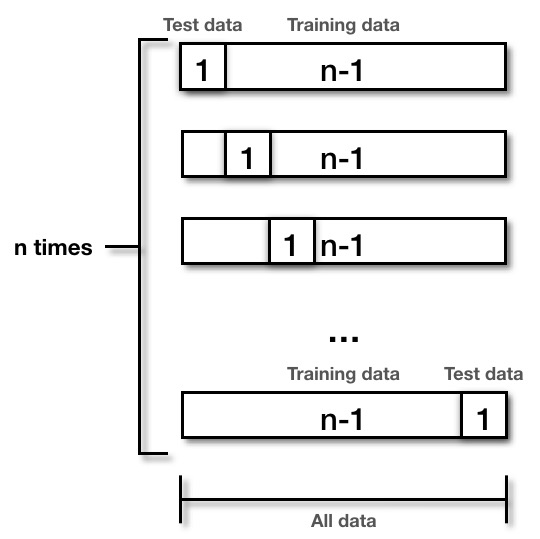
\includegraphics[width=8.5cm, angle=0]{cross-validation.png}  % width changes size
	    \vspace*{-0.25cm}    % manual adjustment of vertical spacing
		\caption{The flow of the cross-validation}          % a meaningful caption
		\label{fig:cross-validation}               % label for the figure
	\end{figure}                        % end of figure environment
	
	The choice between LOO and k-fold cross-validation is determined according to the number of samples. When the sample size is small, the LOO is preferred. When the sample size is too large, the k-fold cross-test is preferred. There is an additional reminder here that the difference between LOO and the k-fold cross-validation is not just a difference in computing time. More, when the sample size is too large, LOO may cause over-fitting problems, and the k-fold cross-validation can not only save computational power, but also avoid the over-fitting problem in here. Chapter \ref{sec:Cross-Validation} will discuss the difference.
	
	\subsection{PLS algorithm}
	\label{PLS_al}
	The partial least squares regression (PLS) is a multi-regression technique proposed by \citet{wold1984collinearity}, and it is also the most common statistical method in the research of near-infrared spectroscopy. Partial least squares regression is similar to principal components analysis (PCA) and is also a factor analysis method. In the modelling  process, it is first necessary to decompose the matrix of spectrum and then extract a few principal components (these variables are called latent variables in PLS) to represent most of the information of original spectrum. Because the spectral data is high-dimensional, the number of independent variables is more than the number of samples, thus it cannot meet the basic assumption of least squares method. Therefore, it is necessary to extracting the data to some components, and then make the regression. Compared with PCA, PLS not only considers the dimensionality reduction of the independent variables, but also maximizes the covariance between the components and target variables. In this way, the covariance between the extracted components and the target vector will be the maximum. From this point, PLS is the improvement and further development of PCA, and the results in many applications also prove that PLS has better performance than PCA.
	
	The process of partial least squares regression is as follows:
	
	The PLS model needs to perform principal component decomposition on the spectral data matrix and the target vector when it is established.
	
	\begin{equation}
	X=TP^T+E 
	\end{equation}
	\begin{equation}
	Y=UQ^T+F
	\end{equation}
	Where T and P are the scoring matrix and the load matrix of the spectral matrix X, respectively. U and Q are the scoring matrix and the load matrix of the detection target vector Y, respectively. E and F are residual matrices of the spectral matrix X and the detection target vector Y, respectively, and T and U can perform linear regression as follows:
	......
	
	\subsection{Parallel computing}
	\label{parallel}
	
	\subsection{High performance computing system}
	\label{myriad}
	
	
	\section{Result and discussion}
	\label{sec:result}
	
	\subsection{Loop times}
	\label{sec:Loop times}
	\begin{figure}[h]    % start of figure environment
		\centering           % put the graph(s) in the centre of the page (horizontally)
		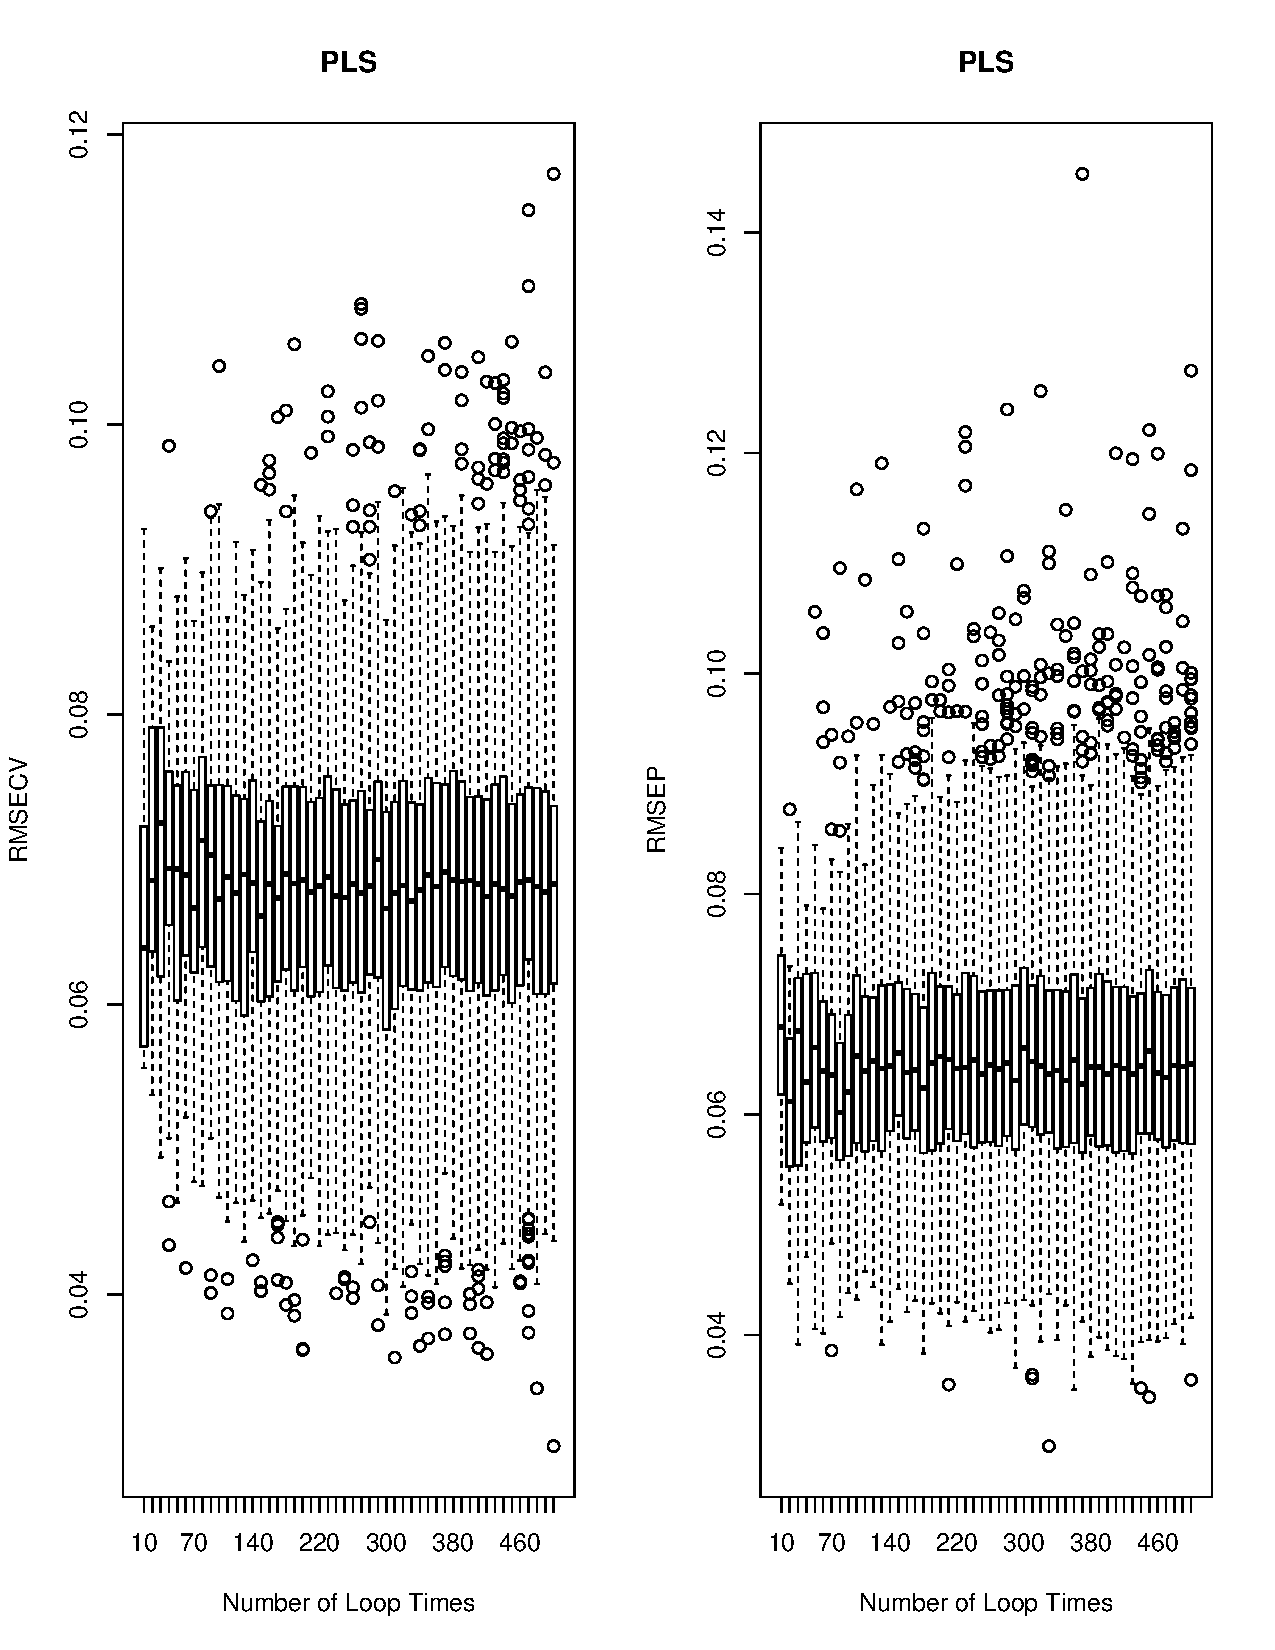
\includegraphics[width=15.5cm, angle=0]{no_loop_time500.pdf}  % width changes size
		\vspace*{-0.25cm}    % manual adjustment of vertical spacing
		\caption{RMSECV and RMSEP under different loop times}          % a meaningful caption
		\label{fig:looptimes}               % label for the figure
	\end{figure}                        % end of figure environment

	\begin{figure}[h]    % start of figure environment
	\centering           % put the graph(s) in the centre of the page (horizontally)
	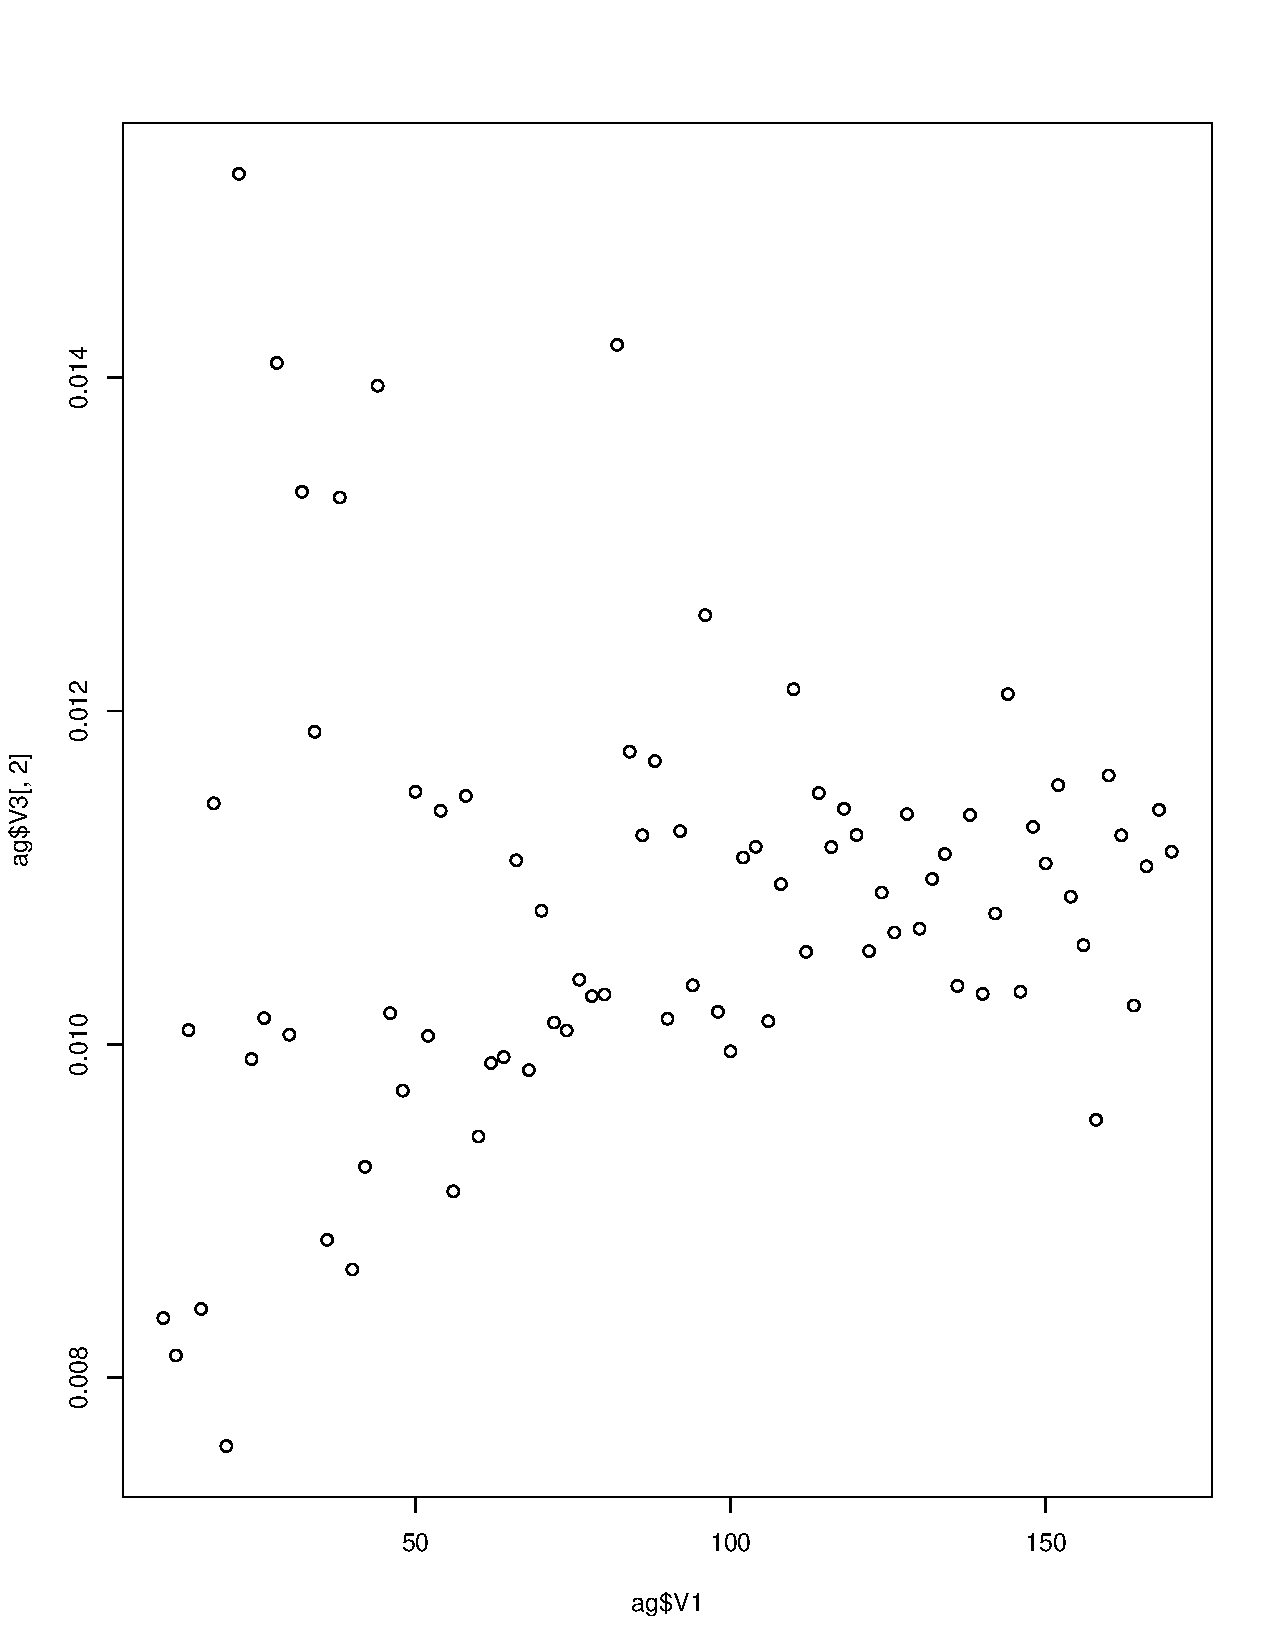
\includegraphics[width=8.5cm, angle=0]{Number_of_loop_times_mp5-1.pdf}  % width changes size
	\vspace*{-0.25cm}    % manual adjustment of vertical spacing
	\caption{SD under different loop times}          % a meaningful caption
	\label{fig:looptimes}               % label for the figure
\end{figure}                        % end of figure environment
	
	\subsection{Number of Samples}
	\label{sec:Number of Samples}
	
	\subsection{Number of Components}
	\label{sec:Number of Components}
	
	\subsection{Pre-treatment}
	\label{sec:Pre-treatment}
	
	\subsection{Cross-Validation}
	\label{sec:Cross-Validation}
	
	\subsection{Compare with papers}
	\label{sec:Compare with papers}
	

	
	\begin{landscape}
		
\begin{table}[]
	\begin{tabular}{lll}
		\hline
		Number & Paper's title & Publication date \\ \hline
		1 & A Partial Least Squares‐Based Consensus Regression Method for the Analysis of Near‐Infrared Complex Spectral Data of Plant Samples & 2007 \\
		2 & A strategy that iteratively retains informative variables for selecting optimal variable subset in multivariate calibration & 2014 \\
		3 & Reduced PCR/PLSR models by subspace projections & 2006 \\
		4 & Stability competitive adaptive reweighted sampling (SCARS) and its applications to multivariate calibration of NIR spectra & 2012 \\
		5 & Cross-validation for the selection of spectral variables using the successive projections algorithm & 2007 \\
		6 & A variable elimination method to improve the parsimony of MLR models using the successive projections algorithm & 2008 \\
		7 & Pretreating near infrared spectra with fractional order Savitzky–Golay differentiation (FOSGD) & 2015 \\
		8 & Using consensus interval partial least square in near infrared spectra analysis & 2015
	\end{tabular}

\label{tab:papers}
\end{table}

Table \ref{tab:moisture} is the regression for moisture.
% Please add the following required packages to your document preamble:
% \usepackage{multirow}
\begin{table}[]
	\begin{tabular}{llllllllllllll}
		\cline{1-11}
		\multicolumn{1}{c}{\multirow{2}{*}{Paper}} & \multicolumn{1}{c}{\multirow{2}{*}{\begin{tabular}[c]{@{}c@{}}Data\\ set\end{tabular}}} & \multicolumn{1}{c}{\multirow{2}{*}{\begin{tabular}[c]{@{}c@{}}Pre-\\ treatment\end{tabular}}} & \multirow{2}{*}{\begin{tabular}[c]{@{}l@{}}Calibration\\ set\end{tabular}} & \multirow{2}{*}{\begin{tabular}[c]{@{}l@{}}Number of\\ Components\end{tabular}} & \multicolumn{2}{c}{Moisture} & \multicolumn{2}{c}{PLS in papers} & \multicolumn{2}{c}{Developed method} &  &  &  \\ \cline{6-11}
		\multicolumn{1}{c}{} & \multicolumn{1}{c}{} & \multicolumn{1}{c}{} &  &  & RMSECV & RMSEP & RMSECV & RMSEP & RMSECV & RMSEP &  &  &  \\ \cline{1-11}
		1 & mp6 & None & 60(LOO) & 10 &  & 0.148(0.0213) &  & 0.159 &  & 0.139 &  &  &  \\
		2 & m5 & None & 64(5-fold) & 10 & 0.0152(0.000739) & 0.0202(0.00319) & 0.0149 & 0.0201 & 0.00026 & 0.00035 &  &  &  \\
		3 & m5 & Scale & 40(LOO) & 12 &  & 0.0231(0.00443) &  & 0.3506 &  & 0.3485 &  &  &  \\
		3 & mp5 & Scale & 40(LOO) & 12 &  & 0.159(0.0178) &  & 0.3506 &  & 0.3485 &  &  &  \\
		4 & mp5 & Scale & 40(LOO) & 10 &  & 0.405(0.0467) &  & 0.357 &  & 0.265 &  &  &  \\
		5 & m5 & SG(1,2,13) & 60(3-fold) & 5 &  & 0.0547(0.00942) &  & 0.040 &  & 0.012 &  &  &  \\
		6 & m5 & SG(1,2,21) & 60(LOO) & 6 &  & 0.0396(0.00625) &  & 0.045 &  & 0.019 &  &  &  \\
		8 & m5 & Delete 75 , 77 & 52(LOO) & 10 & 0.0221(0.0018) & 0.0194(0.00298) & 0.0124 & 0.0157 & 0.0047 & 0.0056 &  &  & 
	\end{tabular}

\caption{regression of moisture}
\label{tab:moisture}
\end{table}

Table \ref{tab:oil} is the regression for Oil.
% Please add the following required packages to your document preamble:
% \usepackage{multirow}
\begin{table}[]
	\begin{tabular}{llllllllllllll}
		\cline{1-11}
		\multicolumn{1}{c}{\multirow{2}{*}{Paper}} & \multicolumn{1}{c}{\multirow{2}{*}{\begin{tabular}[c]{@{}c@{}}Data\\ set\end{tabular}}} & \multicolumn{1}{c}{\multirow{2}{*}{\begin{tabular}[c]{@{}c@{}}Pre-\\ treatment\end{tabular}}} & \multirow{2}{*}{\begin{tabular}[c]{@{}l@{}}Calibration\\ set\end{tabular}} & \multirow{2}{*}{\begin{tabular}[c]{@{}l@{}}Number of\\ Components\end{tabular}} & \multicolumn{2}{c}{Oil} & \multicolumn{2}{c}{PLS in papers} & \multicolumn{2}{c}{Developed method} &  &  &  \\ \cline{6-11}
		\multicolumn{1}{c}{} & \multicolumn{1}{c}{} & \multicolumn{1}{c}{} &  &  & RMSECV & RMSEP & RMSECV & RMSEP & RMSECV & RMSEP &  &  &  \\ \cline{1-11}
		1 & mp6 & None & 60(LOO) & 10 &  & 0.0991(0.0161) &  & 0.107 &  & 0.0948 &  &  &  \\
		3 & m5 & Scale & 40(LOO) & 14 &  & 0.396(0.0665) &  & 0.6912 &  & 0.6902 &  &  &  \\
		3 & mp5 & Scale & 40(LOO) & 14 &  & 0.694(0.095) &  & 0.6912 &  & 0.6902 &  &  &  \\
		5 & m5 & SG(1,2,13) & 60(3-fold) & 12 &  & 0.0329(0.00672) &  & 0.029 &  & 0.022 &  &  &  \\
		6 & m5 & SG(1,2,21) & 60(LOO) & 10 &  & 0.0505(0.0103) &  & 0.028 &  & 0.030 &  &  &  \\
		7 & m5 & SG(0,2,13) & 64(5-fold) & 7 & 0.0827(0.00419) & 0.0716(0.0116) & 0.0729 & 0.0855 & 0.0363 & 0.0400 &  &  &  \\
		7 & m5 & SG(1,2,13) & 64(5-fold) & 7 & 0.0639(0.00357) & 0.0548(0.012) & 0.0577 & 0.0682 & 0.0363 & 0.0400 &  &  &  \\
		7 & m5 & SG(2,2,13) & 64(5-fold) & 7 & 0.0480(0.00312) & 0.0368 (0.0088) & 0.0370 & 0.0397 & 0.0363 & 0.0400 &  &  &  \\
		8 & m5 & Delete 75 , 77 & 52(LOO) & 10 & 0.0651(0.00662) & 0.0604(0.00876) & 0.0613 & 0.0673 & 0.0483 & 0.0546 &  &  & 
	\end{tabular}

\caption{regression of oil}
\label{tab:oil}
\end{table}
    \end{landscape}

	\begin{landscape}
Table \ref{tab:protein} is the regression for protein.
% Please add the following required packages to your document preamble:
% \usepackage{multirow}
\begin{table}[]
	\begin{tabular}{llllllllllllll}
		\cline{1-11}
		\multicolumn{1}{c}{\multirow{2}{*}{Paper}} & \multicolumn{1}{c}{\multirow{2}{*}{\begin{tabular}[c]{@{}c@{}}Data\\ set\end{tabular}}} & \multicolumn{1}{c}{\multirow{2}{*}{\begin{tabular}[c]{@{}c@{}}Pre-\\ treatment\end{tabular}}} & \multirow{2}{*}{\begin{tabular}[c]{@{}l@{}}Calibration\\ set\end{tabular}} & \multirow{2}{*}{\begin{tabular}[c]{@{}l@{}}Number of\\ Components\end{tabular}} & \multicolumn{2}{c}{Protein} & \multicolumn{2}{c}{PLS in papers} & \multicolumn{2}{c}{Developed method} &  &  &  \\ \cline{6-11}
		\multicolumn{1}{c}{} & \multicolumn{1}{c}{} & \multicolumn{1}{c}{} &  &  & RMSECV & RMSEP & RMSECV & RMSEP & RMSECV & RMSEP &  &  &  \\ \cline{1-11}
		1 & mp6 & None & 60(LOO) & 10 &  & 0.141(0.0203) &  & 0.150 &  & 0.145 &  &  &  \\
		3 & m5 & Scale & 40(LOO) & 8 &  & 0.349(0.051) &  & 0.4466 &  & 0.4349 &  &  &  \\
		3 & mp5 & Scale & 40(LOO) & 8 &  & 0.37(0.0485) &  & 0.4466 &  & 0.4349 &  &  &  \\
		5 & m5 & SG(1,2,13) & 60(3-fold) & 6 &  & 0.107(0.0195) &  & 0.119 &  & 0.040 &  &  &  \\
		6 & m5 & SG(1,2,21) & 60(LOO) & 7 &  & 0.102(0.0186) &  & 0.110 &  & 0.033 &  &  &  \\
		8 & m5 & Delete 75 , 77 & 52(LOO) & 13 & 0.119(0.0155) & 0.11(0.0169) & 0.1080 & 0.1353 & 0.0429 & 0.0846 &  &  & 
	\end{tabular}
\caption{regression of protein}
\label{tab:protein}
\end{table}


Table \ref{tab:starch} is the regression for starch.
% Please add the following required packages to your document preamble:
% \usepackage{multirow}
\begin{table}[]
	\begin{tabular}{llllllllllllll}
		\cline{1-11}
		\multicolumn{1}{c}{\multirow{2}{*}{Paper}} & \multicolumn{1}{c}{\multirow{2}{*}{\begin{tabular}[c]{@{}c@{}}Data\\ set\end{tabular}}} & \multicolumn{1}{c}{\multirow{2}{*}{\begin{tabular}[c]{@{}c@{}}Pre-\\ treatment\end{tabular}}} & \multirow{2}{*}{\begin{tabular}[c]{@{}l@{}}Calibration\\ set\end{tabular}} & \multirow{2}{*}{\begin{tabular}[c]{@{}l@{}}Number of\\ Components\end{tabular}} & \multicolumn{2}{c}{Starch} & \multicolumn{2}{c}{PLS in papers} & \multicolumn{2}{c}{Developed method} &  &  &  \\ \cline{6-11}
		\multicolumn{1}{c}{} & \multicolumn{1}{c}{} & \multicolumn{1}{c}{} &  &  & RMSECV & RMSEP & RMSECV & RMSEP & RMSECV & RMSEP &  &  &  \\ \cline{1-11}
		1 & mp6 & None & 60(LOO) & 10 &  & 0.35(0.056) &  & 0.370 &  & 0.358 &  &  &  \\
		3 & m5 & Scale & 40(LOO) & 9 &  & 0.393(0.0736) &  & 0.5010 &  & 0.4443 &  &  &  \\
		3 & mp5 & Scale & 40(LOO) & 9 &  & 0.513(0.0779) &  & 0.5010 &  & 0.4443 &  &  &  \\
		5 & m5 & SG(1,2,13) & 60(3-fold) & 6 &  & 0.239(0.0449) &  & 0.196 &  & 0.100 &  &  &  \\
		6 & m5 & SG(1,2,21) & 60(LOO) & 5 &  & 0.258(0.0453) &  & 0.228 &  & 0.101 &  &  &  \\
		7 & m5 & SG(0,2,13) & 64(5-fold) & 8 & 0.333(0.0226) & 0.283(0.0624) & 0.312 & 0.214 & 0.240 & 0.219 &  &  &  \\
		7 & m5 & SG(1,2,13) & 64(5-fold) & 8 & 0.2412(0.0171) & 0.221(0.049) & 0.248 & 0.221 & 0.240 & 0.219 &  &  &  \\
		7 & m5 & SG(2,2,13) & 64(5-fold) & 8 & 0.318(0.0252) & 0.302(0.061) & 0.347 & 0.228 & 0.240 & 0.219 &  &  &  \\
		8 & m5 & Delete 75 , 77 & 52(LOO) & 10 & 0.292(0.0312) & 0.282(0.043) & 0.2579 & 0.2356 & 0.1137 & 0.1188 &  &  & 
	\end{tabular}
\caption{regression of starch}
\label{tab:starch}
\end{table}
    \end{landscape}

	\section{Conclusions}
	\label{sec:conclution}
	
	
	
	
	
	

	
	\addcontentsline{toc}{section}{References} % to add references to table of contents
	\bibliography{hongwei_pls_MSc}                     % read references from example.bib
	\bibliographystyle{chicago}            % file to determine the style of references
	
\end{document} 